% Created by tikzDevice version 0.12 on 2019-01-03 18:24:28
% !TEX encoding = UTF-8 Unicode
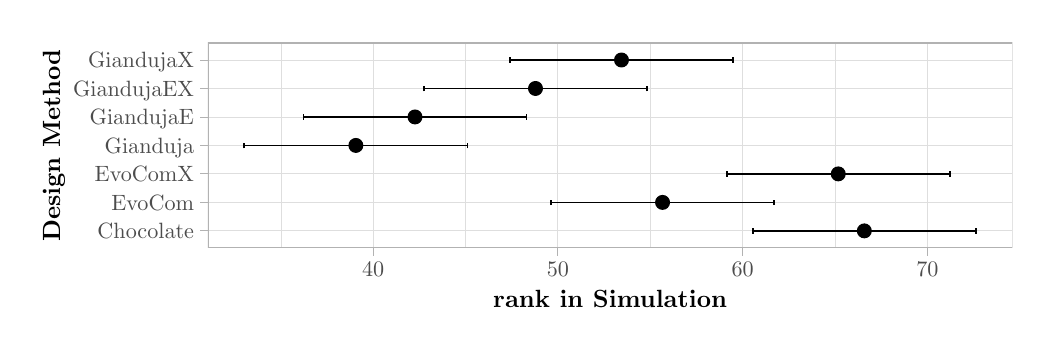
\begin{tikzpicture}[x=1pt,y=1pt]
\definecolor{fillColor}{RGB}{255,255,255}
\path[use as bounding box,fill=fillColor,fill opacity=0.00] (0,0) rectangle (361.35,108.41);
\begin{scope}
\path[clip] (  0.00,  0.00) rectangle (361.35,108.40);
\definecolor{drawColor}{RGB}{255,255,255}
\definecolor{fillColor}{RGB}{255,255,255}

\path[draw=drawColor,line width= 0.6pt,line join=round,line cap=round,fill=fillColor] (  0.00,  0.00) rectangle (361.35,108.40);
\end{scope}
\begin{scope}
\path[clip] ( 65.07, 28.81) rectangle (355.85,102.90);
\definecolor{fillColor}{RGB}{255,255,255}

\path[fill=fillColor] ( 65.07, 28.81) rectangle (355.85,102.90);
\definecolor{drawColor}{gray}{0.87}

\path[draw=drawColor,line width= 0.1pt,line join=round] ( 91.45, 28.81) --
	( 91.45,102.90);

\path[draw=drawColor,line width= 0.1pt,line join=round] (158.20, 28.81) --
	(158.20,102.90);

\path[draw=drawColor,line width= 0.1pt,line join=round] (224.96, 28.81) --
	(224.96,102.90);

\path[draw=drawColor,line width= 0.1pt,line join=round] (291.72, 28.81) --
	(291.72,102.90);

\path[draw=drawColor,line width= 0.3pt,line join=round] ( 65.07, 34.98) --
	(355.85, 34.98);

\path[draw=drawColor,line width= 0.3pt,line join=round] ( 65.07, 45.27) --
	(355.85, 45.27);

\path[draw=drawColor,line width= 0.3pt,line join=round] ( 65.07, 55.57) --
	(355.85, 55.57);

\path[draw=drawColor,line width= 0.3pt,line join=round] ( 65.07, 65.86) --
	(355.85, 65.86);

\path[draw=drawColor,line width= 0.3pt,line join=round] ( 65.07, 76.15) --
	(355.85, 76.15);

\path[draw=drawColor,line width= 0.3pt,line join=round] ( 65.07, 86.44) --
	(355.85, 86.44);

\path[draw=drawColor,line width= 0.3pt,line join=round] ( 65.07, 96.73) --
	(355.85, 96.73);

\path[draw=drawColor,line width= 0.3pt,line join=round] (124.82, 28.81) --
	(124.82,102.90);

\path[draw=drawColor,line width= 0.3pt,line join=round] (191.58, 28.81) --
	(191.58,102.90);

\path[draw=drawColor,line width= 0.3pt,line join=round] (258.34, 28.81) --
	(258.34,102.90);

\path[draw=drawColor,line width= 0.3pt,line join=round] (325.09, 28.81) --
	(325.09,102.90);
\definecolor{drawColor}{RGB}{0,0,0}
\definecolor{fillColor}{RGB}{0,0,0}

\path[draw=drawColor,line width= 0.4pt,line join=round,line cap=round,fill=fillColor] (302.32, 34.98) circle (  2.50);

\path[draw=drawColor,line width= 0.4pt,line join=round,line cap=round,fill=fillColor] (229.41, 45.27) circle (  2.50);

\path[draw=drawColor,line width= 0.4pt,line join=round,line cap=round,fill=fillColor] (292.90, 55.57) circle (  2.50);

\path[draw=drawColor,line width= 0.4pt,line join=round,line cap=round,fill=fillColor] (118.59, 65.86) circle (  2.50);

\path[draw=drawColor,line width= 0.4pt,line join=round,line cap=round,fill=fillColor] (139.96, 76.15) circle (  2.50);

\path[draw=drawColor,line width= 0.4pt,line join=round,line cap=round,fill=fillColor] (183.50, 86.44) circle (  2.50);

\path[draw=drawColor,line width= 0.4pt,line join=round,line cap=round,fill=fillColor] (214.57, 96.73) circle (  2.50);

\path[draw=drawColor,line width= 0.6pt,line join=round] (342.63, 33.95) --
	(342.63, 36.01);

\path[draw=drawColor,line width= 0.6pt,line join=round] (342.63, 34.98) --
	(262.01, 34.98);

\path[draw=drawColor,line width= 0.6pt,line join=round] (262.01, 33.95) --
	(262.01, 36.01);

\path[draw=drawColor,line width= 0.6pt,line join=round] (269.72, 44.25) --
	(269.72, 46.30);

\path[draw=drawColor,line width= 0.6pt,line join=round] (269.72, 45.27) --
	(189.10, 45.27);

\path[draw=drawColor,line width= 0.6pt,line join=round] (189.10, 44.25) --
	(189.10, 46.30);

\path[draw=drawColor,line width= 0.6pt,line join=round] (333.21, 54.54) --
	(333.21, 56.59);

\path[draw=drawColor,line width= 0.6pt,line join=round] (333.21, 55.57) --
	(252.59, 55.57);

\path[draw=drawColor,line width= 0.6pt,line join=round] (252.59, 54.54) --
	(252.59, 56.59);

\path[draw=drawColor,line width= 0.6pt,line join=round] (158.90, 64.83) --
	(158.90, 66.89);

\path[draw=drawColor,line width= 0.6pt,line join=round] (158.90, 65.86) --
	( 78.28, 65.86);

\path[draw=drawColor,line width= 0.6pt,line join=round] ( 78.28, 64.83) --
	( 78.28, 66.89);

\path[draw=drawColor,line width= 0.6pt,line join=round] (180.27, 75.12) --
	(180.27, 77.18);

\path[draw=drawColor,line width= 0.6pt,line join=round] (180.27, 76.15) --
	( 99.65, 76.15);

\path[draw=drawColor,line width= 0.6pt,line join=round] ( 99.65, 75.12) --
	( 99.65, 77.18);

\path[draw=drawColor,line width= 0.6pt,line join=round] (223.81, 85.41) --
	(223.81, 87.47);

\path[draw=drawColor,line width= 0.6pt,line join=round] (223.81, 86.44) --
	(143.19, 86.44);

\path[draw=drawColor,line width= 0.6pt,line join=round] (143.19, 85.41) --
	(143.19, 87.47);

\path[draw=drawColor,line width= 0.6pt,line join=round] (254.88, 95.70) --
	(254.88, 97.76);

\path[draw=drawColor,line width= 0.6pt,line join=round] (254.88, 96.73) --
	(174.26, 96.73);

\path[draw=drawColor,line width= 0.6pt,line join=round] (174.26, 95.70) --
	(174.26, 97.76);
\definecolor{drawColor}{gray}{0.70}

\path[draw=drawColor,line width= 0.6pt,line join=round,line cap=round] ( 65.07, 28.81) rectangle (355.85,102.90);
\end{scope}
\begin{scope}
\path[clip] (  0.00,  0.00) rectangle (361.35,108.41);
\definecolor{drawColor}{gray}{0.30}

\node[text=drawColor,anchor=base east,inner sep=0pt, outer sep=0pt, scale=  0.80] at ( 60.12, 32.23) {Chocolate};

\node[text=drawColor,anchor=base east,inner sep=0pt, outer sep=0pt, scale=  0.80] at ( 60.12, 42.52) {EvoCom};

\node[text=drawColor,anchor=base east,inner sep=0pt, outer sep=0pt, scale=  0.80] at ( 60.12, 52.81) {EvoComX};

\node[text=drawColor,anchor=base east,inner sep=0pt, outer sep=0pt, scale=  0.80] at ( 60.12, 63.10) {Gianduja};

\node[text=drawColor,anchor=base east,inner sep=0pt, outer sep=0pt, scale=  0.80] at ( 60.12, 73.39) {GiandujaE};

\node[text=drawColor,anchor=base east,inner sep=0pt, outer sep=0pt, scale=  0.80] at ( 60.12, 83.68) {GiandujaEX};

\node[text=drawColor,anchor=base east,inner sep=0pt, outer sep=0pt, scale=  0.80] at ( 60.12, 93.98) {GiandujaX};
\end{scope}
\begin{scope}
\path[clip] (  0.00,  0.00) rectangle (361.35,108.41);
\definecolor{drawColor}{gray}{0.70}

\path[draw=drawColor,line width= 0.3pt,line join=round] ( 62.32, 34.98) --
	( 65.07, 34.98);

\path[draw=drawColor,line width= 0.3pt,line join=round] ( 62.32, 45.27) --
	( 65.07, 45.27);

\path[draw=drawColor,line width= 0.3pt,line join=round] ( 62.32, 55.57) --
	( 65.07, 55.57);

\path[draw=drawColor,line width= 0.3pt,line join=round] ( 62.32, 65.86) --
	( 65.07, 65.86);

\path[draw=drawColor,line width= 0.3pt,line join=round] ( 62.32, 76.15) --
	( 65.07, 76.15);

\path[draw=drawColor,line width= 0.3pt,line join=round] ( 62.32, 86.44) --
	( 65.07, 86.44);

\path[draw=drawColor,line width= 0.3pt,line join=round] ( 62.32, 96.73) --
	( 65.07, 96.73);
\end{scope}
\begin{scope}
\path[clip] (  0.00,  0.00) rectangle (361.35,108.41);
\definecolor{drawColor}{gray}{0.70}

\path[draw=drawColor,line width= 0.3pt,line join=round] (124.82, 26.06) --
	(124.82, 28.81);

\path[draw=drawColor,line width= 0.3pt,line join=round] (191.58, 26.06) --
	(191.58, 28.81);

\path[draw=drawColor,line width= 0.3pt,line join=round] (258.34, 26.06) --
	(258.34, 28.81);

\path[draw=drawColor,line width= 0.3pt,line join=round] (325.09, 26.06) --
	(325.09, 28.81);
\end{scope}
\begin{scope}
\path[clip] (  0.00,  0.00) rectangle (361.35,108.41);
\definecolor{drawColor}{gray}{0.30}

\node[text=drawColor,anchor=base,inner sep=0pt, outer sep=0pt, scale=  0.80] at (124.82, 18.35) {40};

\node[text=drawColor,anchor=base,inner sep=0pt, outer sep=0pt, scale=  0.80] at (191.58, 18.35) {50};

\node[text=drawColor,anchor=base,inner sep=0pt, outer sep=0pt, scale=  0.80] at (258.34, 18.35) {60};

\node[text=drawColor,anchor=base,inner sep=0pt, outer sep=0pt, scale=  0.80] at (325.09, 18.35) {70};
\end{scope}
\begin{scope}
\path[clip] (  0.00,  0.00) rectangle (361.35,108.41);
\definecolor{drawColor}{RGB}{0,0,0}

\node[text=drawColor,anchor=base,inner sep=0pt, outer sep=0pt, scale=  0.90] at (210.46,  7.44) {\bfseries rank in Simulation};
\end{scope}
\begin{scope}
\path[clip] (  0.00,  0.00) rectangle (361.35,108.41);
\definecolor{drawColor}{RGB}{0,0,0}

\node[text=drawColor,rotate= 90.00,anchor=base,inner sep=0pt, outer sep=0pt, scale=  0.90] at ( 11.71, 65.86) {\bfseries Design Method};
\end{scope}
\end{tikzpicture}
